\chapter{Teorema de \emph{Noether} II/II}
\label{NoetherIIdeII}

	
\begin{tikzpicture}
	\fill [left color=red!50, right color=teal!50] (0,0) rectangle (6.5,.1);
	\fill [left color=teal!50, right color=blue!50] (6.5,0) rectangle (11.5,.1);
	\end{tikzpicture}



\vspace{10mm}
\begin{adjustwidth}{50pt}{50pt}
\begin{ejemplo}
\begin{multicols}{2}

$\,$

En este capítulo veremos es teorema de Noether de forma precisa y seguiremos con el ejemplo de tema anterior. 

Antes repasaremos lo que se entiende por \emph{deivada direccional}, importantísima en el teorema de Noether.

$\,$
\begin{figure}[H]
	\centering
	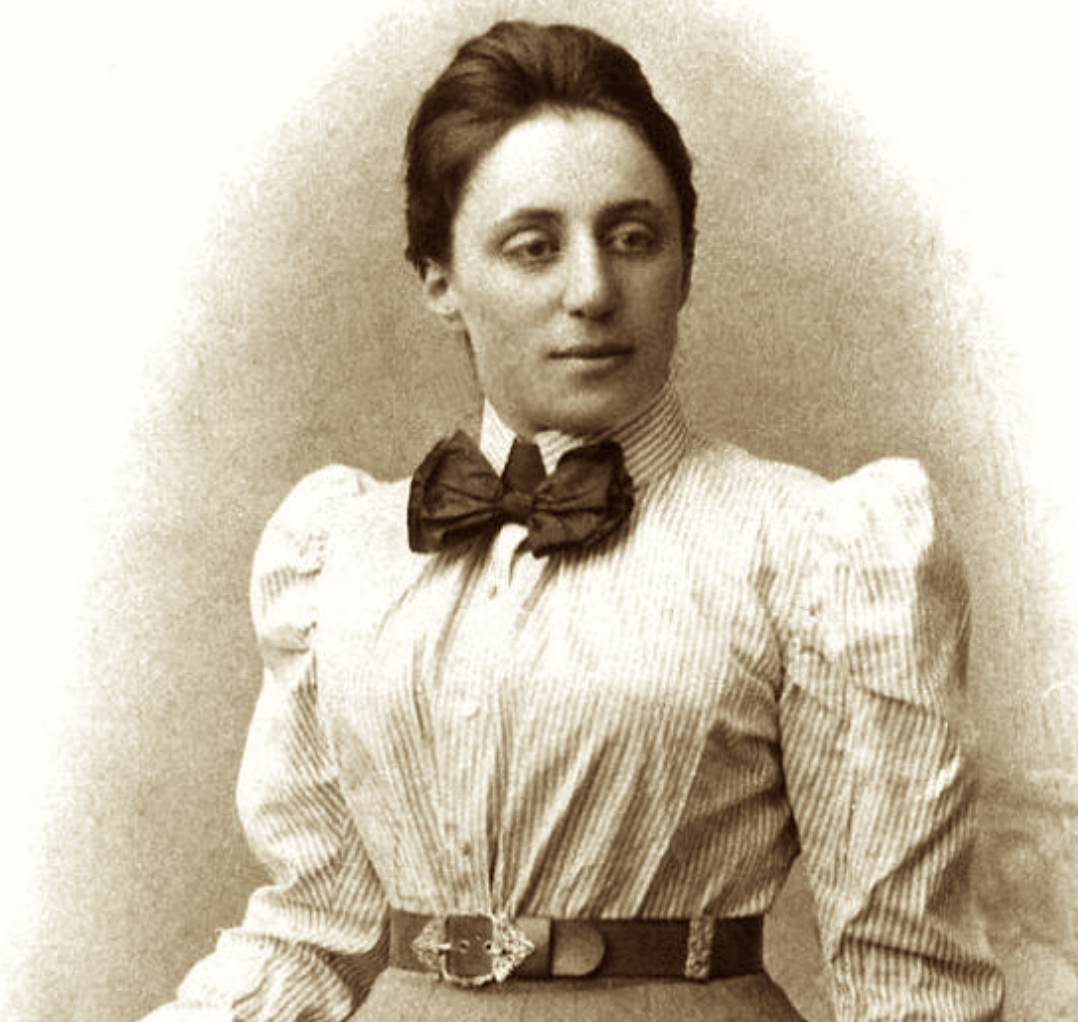
\includegraphics[width=.4\textwidth]{imagenes/img14-01.png}
\end{figure}

\end{multicols}
\end{ejemplo}
\end{adjustwidth}
\vspace{5mm}

\section{La derivada direccional}

Consideremos una función de dos variables $f(x,y)=x^2+y^2$, por ejemplo, y supongamos que pasamos del punto $A(1,1)$ a otro muy próximo a $B(1.01,1)$ en su misma horizontal, dirección $\vec n=(1,0)$. 

La variación de la función al pasar de $A$ a $B$ es $\ \Delta f=f(B)-f(A)=f(1.01,1)-f(1,1)=0.0201$

Podemos interpretar esto como $\quad \dfrac{\Delta f}{\Delta x}\ \Delta x=\dfrac{0.0201}{0.01} \ 0.01=0.0201 \quad $ y, para $ \quad \Delta x <<1 \quad $ llamar $ \displaystyle \pdv{f}{x}=\dfrac{\Delta f}{\Delta x}=\dfrac{0.0201}{0.01}=2.01\,; \qquad $ es decir, $\quad \displaystyle \delta F=\pdv{f}{x} \ \var x$

Si $B$ no está en la dirección horizontal a $A$, por ejemplo, si $A(x,y)$ y $B(x+\var x, y+\var y)$, tendremos que 

$\ \displaystyle \var f=f(B)-f(A)=f(x+\var x, y+\var y)-f(x,y)= f(x+\var x, y+\var y)  \textcolor{red}{-f(x,y+\var y)+f(x,y+\var y)} -f(x,y)$

$\var f = \displaystyle
\dfrac{f(x+\var x,y+\var y)-f(x,y+\var y)}{\var x}\var x + \dfrac{f(x,y+\var y)-f(x,y)}{\var y}\var y = \eval{\pdv{f}{x}}_{(x,y+\var y)}\var x +\eval{\pdv{f}{y}}_{(x,y)}\var y $


Para $\var x,\ \var y$ infinitesimales, $\quad  \subrayado{\boldsymbol{ \displaystyle \var f \ = \ \pdv{f}{x} \ \var x \ + \ \pdv{f}{y} \ \var y}}$

\vspace{5mm} 
\begin{multicols}{2}
$\vec \varepsilon \ || \ \vec n \ \to \ \vec n = k \vec \varepsilon$

$\vec n =(n_x,n_y)=k \ (\var x, \var y) \ \to \ \begin{cases} \ n_x=k \ \var x \\ \ n_y=k \ \var y \end{cases}$

$\displaystyle \boldsymbol{ \var f} \ = \ \dfrac 1 k \ \left[ n_x \ \pdv{f}{x} + n_y \ \pdv{f}{y} \right] \ = \ \boldsymbol{\dfrac 1 k \ \vec n \cdot \overrightarrow {\nabla} f}$

El cambio de la función $f$ en una dirección $\vec n$ es igual al producto escalar de $\vec n$ (vector dirección del cambio) por el gradiente de la función $g$.
\begin{figure}[H]
	\centering
	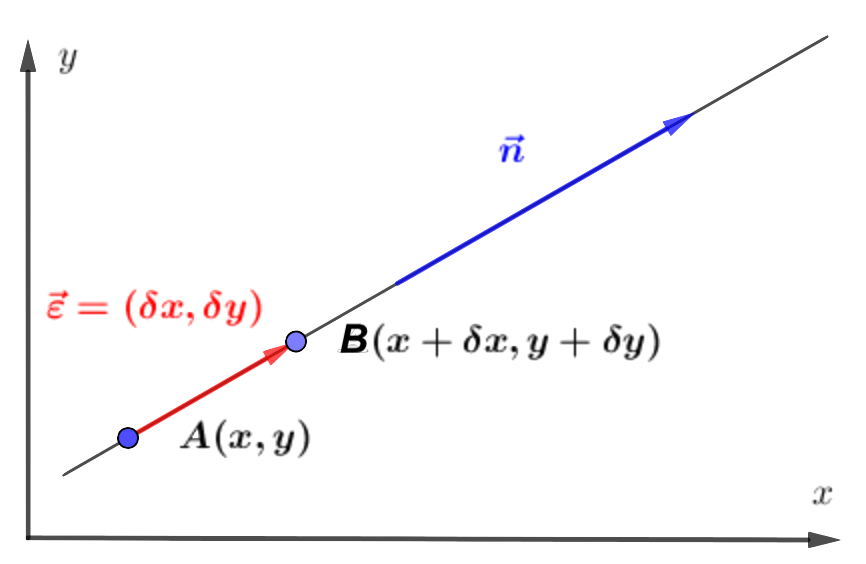
\includegraphics[width=.45\textwidth]{imagenes/img15-01.png}
\end{figure}

\end{multicols}

\vspace{5mm}
\begin{destacado}
	\begin{center} \textbf{$\boldsymbol{\vec n \cdot \overrightarrow {\nabla}} \, , \ $ es la \emph{derivada direccional} de la función $f$ en la dirección $\vec n$.} \end{center}
\end{destacado}

\vspace{5mm}
Veamos un ejemplo de la derivada direccional aplicada a nuestra función $f(x,y)=x^2+y^2$, simetría cilíndrica.

\begin{multicols}{2}
\begin{figure}[H]
	\centering
	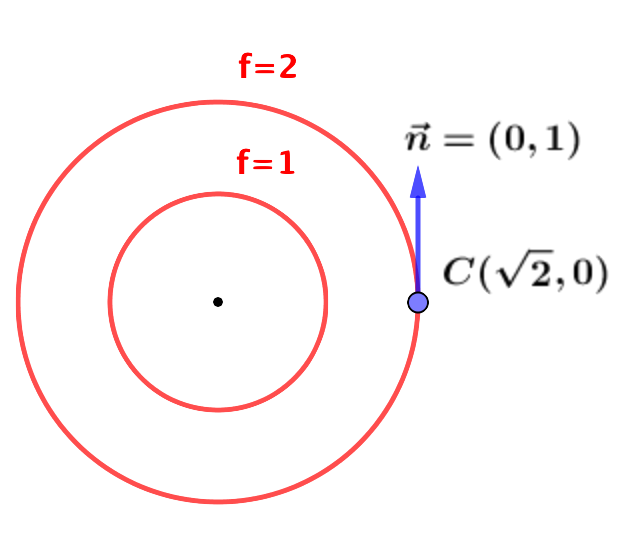
\includegraphics[width=.45\textwidth]{imagenes/img15-02.png}
\end{figure}
Para $r=1,\ x^2+y^2=1 \to f=1$; para $r=\sqrt
2,\ x^2+y^2=2 \to f=2$, son las curvas de nivel de la función $f$.

Situados en la posición $C(\sqrt{2},0)$, la derivada en la dirección tangente, $\vec n=(0.1)$ para un cambio infinitesimal en $C$ es:

$\displaystyle \eval{\var f}_{(\sqrt{2},0)}=\vec n \cdot \overrightarrow \nabla f =(0,1)\cdot (2x,2y)=\eval{0+2y}_{(\sqrt{2},0)}=0$
\end{multicols}


\section {Teorema de \emph{Noether}}

\begin{equation}
\label{T15TNtranf}
f(x_1,x_2,\cdots ,x_N) \quad \to \qquad 	\var f \ = \ \vec n \cdot \overrightarrow \nabla f \ ; \qquad 	\qquad 
\begin{cases}
\ \vec n &= \ (n_1,n_2, \cdots, n_N) \\ \ \overrightarrow \nabla &=\ \displaystyle
\left( \pdv{x_1}, \pdv{x_2}, \cdots , \pdv{x_N} \right)	
\end{cases}
\end{equation}

\begin{figure}[H]
	\centering
	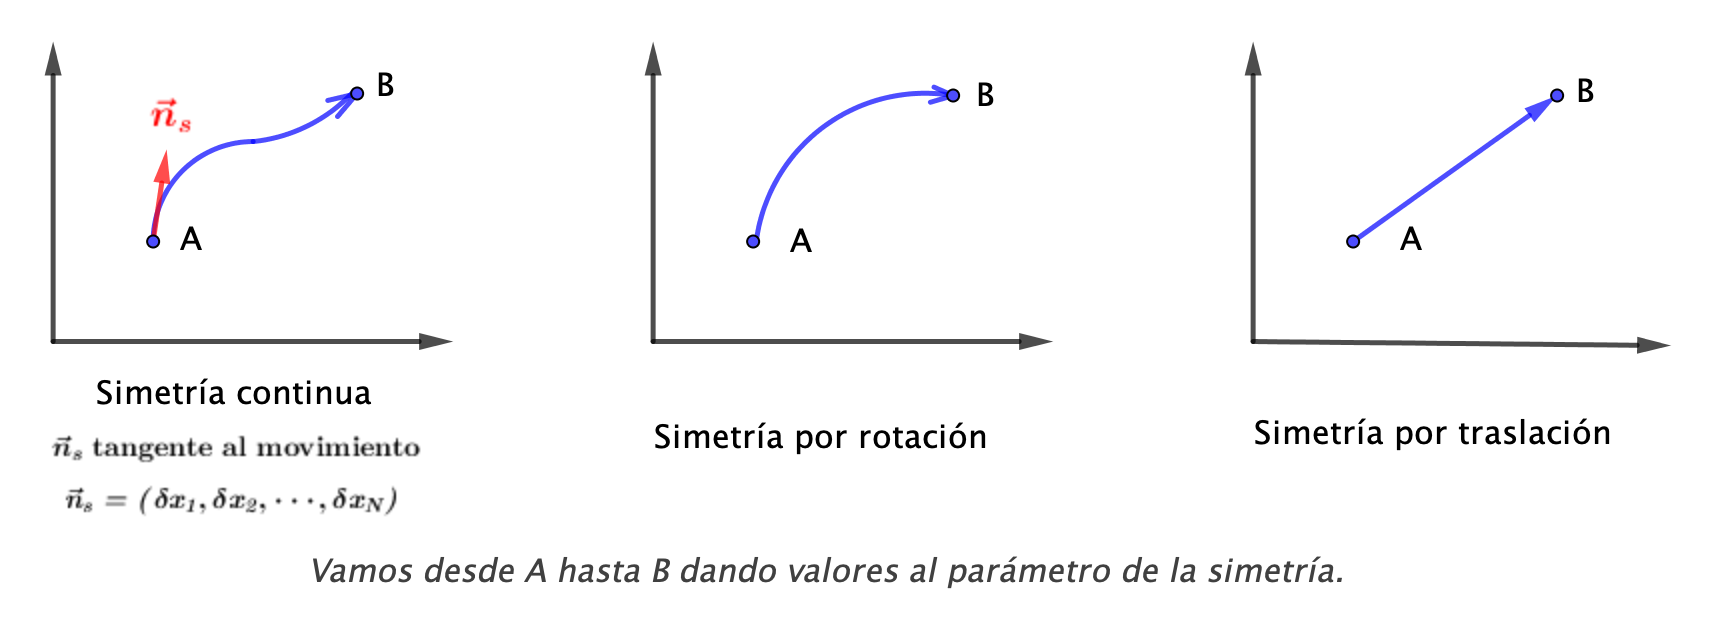
\includegraphics[width=.95\textwidth]{imagenes/img15-03.png}
\end{figure}

La variación de una función $f$ siguiendo la simetría $S$ es:

$(\var f)_S \ = \ \vec n_s \cdot \overrightarrow \nabla f \ = \
\displaystyle
(\var x_1)_S \ \pdv{f}{x_1} + \cdots + (\var x_N)_S \ \pdv{f}{x_N}$

Volviendo a mecánica lagrangiana, $ f(x_1,x_2,x_3) = L(x.\dot x, t)\, , \ $ luego

\begin{equation}
\label{T15ecaucion1}
(\var L)_S \ = \ \displaystyle
\left( \pdv{L}{x} \right)_S \ \var x +
\left( \pdv{L}{\dot x} \right)_S \ \var \dot x +
\left( \pdv{L}{t} \right)_S \ \var t 
\end{equation}

En el ejemplo de simetría del capítulo anterior, 

$\var t=\varepsilon 2t;\qquad \var x= \varepsilon (x-2\dot x t) \ \to \dv{t}:\quad \var \dot x=\varepsilon(\dot x-2\ddot xt-2\dot x)=\varepsilon (-\dot x-2\ddot x t)$

Como, además, $\ L=\dfrac m 2 \dot x^2 - \dfrac {a}{x^2}$, sustituyendo en la ec. \ref{T15ecaucion1}, llegamos en el capítulo 14 a que

\vspace{5mm} $(\var L)_S \ = \ \varepsilon \ \displaystyle \dv{t} [-2tL]$. Resultado obtenido con la simetría del capítulo anterior, para otras simetrías se llega a otros resultados, a una derivada temporal de una cantidad que se le suele llamar $\ \boldsymbol{K=-2tL}$, así, engeneral y para cualquier simetría se tendrá:

\begin{equation}
\label{T15paraTN1}	
(\var L)_S \ = \ \varepsilon \ \dv{t} [K]
\end{equation}

\vspace{5mm} Si queremos calcular la variación del laranginao pero imponiendo solo que se cumplan las ecuaciones de Euler-Lagrange, $(\var L)_{E-L}$ y no exigimos nada al vector $\vec n$ (no imponenmos ninguna restricción de simetría), $\var x, \var y, \var x$ puede ser cualsquiera y se llega (ver capítulo anterior) a:

\begin{equation}
\label{T15paraTN2}	
(\var L)_{E-L} \ = \  \dv{t} \left( \pdv{L}{\dot x} \ \var x \right) \ + \ \var t \ \pdv{L}{t}
\end{equation}

\vspace{5mm}
\begin{ejercicio}
\vspace{2mm}
\begin{multicols}{2}

	\begin{equation}
	\tag{\ref{T15paraTN1}}	
	(\var L)_S \ = \ \varepsilon \ \dv{t} [K]
	\end{equation}
	
	\begin{center}
	\vspace{-5mm} Simetría
	
	\vspace{-3mm} $x(t)$ cualesquiera
	\end{center}
	
	\begin{equation}
	\tag{\ref{T15paraTN2}}	
	(\var L)_{E-L} \ = \  \dv{t} \left( \pdv{L}{\dot x} \ \var x \right) \ + \ \var t \ \pdv{L}{t}
	\end{equation}	
	
	\begin{center}
	\vspace{-5mm} No simetría
	
	\vspace{-3mm} $x(t)$ Euler- Lagrange
	\end{center}

\end{multicols}	
\vspace{2mm}
\end{ejercicio}

\vspace{5mm}
Ambas ecuaciones son independientes. Noether hizo imponer la simetría y las ecuaciones de Euler-Lagrange para ambas $\ \Rightarrow \ (\var L)_S = (\var L)_{E-L}$

\vspace{10mm}
\begin{myblock}{Teorema de Noether para 1-dimensión}
\begin{large}
\begin{equation}
\label{T15ThNoether1-dim}	
	\subrayado{
	\boxed{\ \boldsymbol{
	\varepsilon \ \dv{K}{t} \ = \ (\var t)_S \ \pdv{L}{t} \ + \ \dv{t} \ \left[ \pdv{L}{\dot x} \ (\var x)_S \right]
	}\ }
	}
\end{equation}
\end{large}
\end{myblock}

\vspace{10mm}
Si $\ K=0 \ \text{ y } \ L\neq L(t) \quad \to \quad \boldsymbol{0 \ = \ \displaystyle \dv{t} \left( \pdv{L}{\dot x} \ \var x_S \right)} \, , $ que es una versión muy simple del teorema de Noether que suele aparecer en muchos textos.

Dada una acción, al hacer la transformación de simetría, la acción ha de quedar invariante (si no es así, no se trata de una simetría), pero para culaquier cambio infinitesimal en la acción, ésta no es cero sino que da $\ \var S=\displaystyle \int_{t_1}^{t_2} \dd t \dv{K}{t} \neq 0$

En la transformación del capítulo anterior, $\ y=\lambda t,\ \tau=\lambda^2t\, , \  $ la acción quedaba invariante, pero esta no era una transformación infinitesimal.

Para \textbf{transformaciones infinitesimales} se cumple $\ \boldsymbol{ \var S=\displaystyle \int_{t_1}^{t_2} \dd t \dv{K}{t} \neq 0} \ $ lo cual nos sirve para saber si estamos ante una simetría. Se entenderá mejor con el siguiente ejemplo.

\vspace{10mm}
\subsection{Continuamos con el ejemplo introductorio del tema anterior}
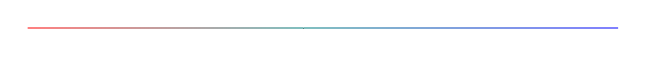
\begin{tikzpicture}
	\fill [left color=red!50, right color=teal!50] (0,0) rectangle (3.5,.01);
	\fill [left color=teal!50, right color=blue!50] (3.5,0) rectangle (7.5,.01);
	\end{tikzpicture}
\vspace{0.5cm}

Desarrollaremos lo que vamos a ver en 6 pasos

\begin{enumerate}
\item Continuamos con nuestro lagrangiano:	$\quad L=\dfrac m 2 \dot x^2 - \dfrac {a}{x^2}$
\item La acción  $s$ es invariante ante la transformación de simetría $\ x\ to \lambda x;\ t\to \lambda^2 t$
\item Hacemos infinitesimal la trensformación de simetría $\ \begin{cases}
 	\ \var t=\varepsilon 2 t \\ \ \var x=\varepsilon (x-2\dot x t) \\ \ \var \dot x = \varepsilon (-\dot x - 2\ddot x t)
 \end{cases}$
 \item Nuestro lagrangiano es, explícitamente, independiente del tiempo: $\ L \neq L(t)$
 
\vspace{5mm} Con todo esto, el teorema de Noether en 1 dimensión queda como:
 
 $$\boldsymbol{\varepsilon \ \displaystyle \dv{K}{t} \ = \ \dv{t} \ \left[ \pdv{L}{\dot x} \ (\var x)_S \right]} $$
 
Integramos, respecto a $t$, ambos lados de la ecuación:
 
\vspace{2mm} $\displaystyle \varepsilon \int \dv{K}{t} \dd t \ = \ \int\dv{t} \ \left[ \pdv{L}{\dot x} \ (\var x)_S \right]\dd t  \quad \to \quad 
0\ =\ \int\dv{t} \ \dd t \ \left[ \pdv{L}{\dot x} \ (\var x)_S  \ - \ \varepsilon K \right]$
  
\vspace{2mm}\vspace{2mm} Como $\var x=\varepsilon (x-2\dot x t)$, en general, $\var x=\varepsilon \ \phi(t,x,\dot x)$, podemos escribir

\vspace{2mm}$\displaystyle 0\ =\ \int\dv{t} \ \dd t \ \left[ \pdv{L}{\dot x} \ \varepsilon \phi(t,x,\dot x)  \ - \ \varepsilon K \right]$, eliminando $\varepsilon$,

\vspace{2mm}$\displaystyle 0\ =\ \int\dv{t} \ \dd t \ \left[ \pdv{L}{\dot x} \ \phi  \ - \  \right] \quad \to \quad
\boxed{\ \boldsymbol{ \pdv{L}{\dot x}\ \phi \ - \ K \ = \ Q } \ } \ \, , \ $ \begin{footnotesize} carga conservada en el caso 1-D y $L\neq L(t)$ \end{footnotesize}
\vspace{2mm}
\item Vamos a averiguar quién es $K$. Usamos nuestra transformación infinitesimal de simetría: 

\vspace{2mm}$\displaystyle L=\dfrac m 2 \dot x^2 -\dfrac{a}{x^2} \ \to \ (\var L)_S=\dfrac m 2 2 \dot x \ \var x - a \left(\dfrac{-2}{x^3} \right) \ \var  x$

\vspace{2mm}\textcolor{gris}{Es como derivar, $x^2 \to 2x \dot x$ pero con \emph{variaciones} $x^2 \to 2x\var x$}

\vspace{2mm}$\displaystyle (\var L)_S=m\dot x \var x + \dfrac{2a}{x^3} \var x$

\vspace{2mm} Imponiendo las condiciones de la simetría (punto 3), tenemos

\vspace{2mm} $\displaystyle (\var L)_S=m\dot x (\dot x -2\ddot x t) + \dfrac{2a}{x^3} (\dot x -2\ddot x t)=\varepsilon \left[ -m\dot x^2-2m\dot x \ddot x t+\dfrac{2a}{x^3}-\dfrac{4a \dot x t}{x^3} \right] = \varepsilon \dv{t} [-2tL]\, , \ $ como vimos en el capítulo anterior.
$\quad (\var L)_S \ = \ \dv{K}{t} \quad \to \quad \boxed{ \ K \ = \ -2tl\ }$

\vspace{2mm}
\item Sustituir $K$ en $Q.\qquad$ \textcolor{gris}{(En nuestro caso, $\ \phi=x-2\dot x t$, visto en punto 4)}

\vspace{2mm} $Q=\displaystyle \pdv{L}{\dot x} \phi - K=m\dot x(x-2\dot xt)+2tL=m\dot x(x-2\dot xt)+2t\left( \dfrac m 2 \dot x^2 -\dfrac{a}{x^2} \right)$

\vspace{2mm}$\displaystyle Q=m\dot x x -2m\dot x^2+m\dot x^2t-\dfrac{2at}{x^2} = m\dot x x -m\dot x^2 t-\dfrac{2at}{x^2}=cte$

\end{enumerate}

\textbf{Veamos un ejemplo numérico para aclararlo un poco más}. En el capítulo anterior encontramos que para nuestro lagrangiano $L=\dfrac m 2 \dot x^2 -\dfrac{a}{x^2}$, la ecuación de movimiento era: $\ x=\sqrt{\dfrac{2}{me}(Q+Et)^2+\dfrac a E}$

Por simplificar, tomamos $m=a=1$ y nos centramos en el punto en que $t=0;\ x=1;\ \dot x=0$. En estas condiciones $Q=0 \text{ y } E=1$, constantes. Particularizando en la ecuación de movimiento (u derivando):

$x=\sqrt{1+2t^2};\quad \dot x=\displaystyle \dv{t} x = \dfrac{2t}{\sqrt{1+2t^2}};\quad \ddot x=\dv{t} \dot x=\dfrac{2}{(1+2t^2)^{3/2}} \ \to \ \ddot x(t=0)=\dfrac 2 1 =2$

\begin{multicols}{2}
En el espacio $\ t,\ x,\ \dot x$ Consideramos el punto $A(0,1,0)$
 \textcolor{gris}{($t=0;\ x=1;\ \dot x=0$)}

Consideramos el vector $\vec n$ que vaya por la simetría, $\vec n_S=( \ (\var x)_S\ , \ (\var y)_S\ , \ (\var z)_S\ )$. 

Nos situamos en el punto inicial A.
\begin{figure}[H]
	\centering
	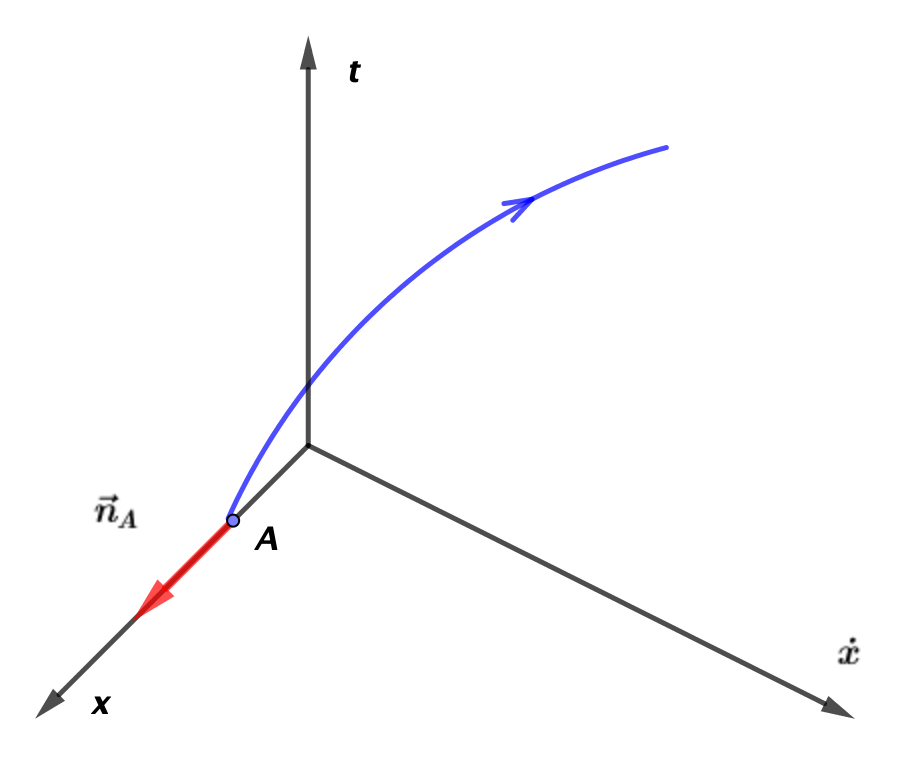
\includegraphics[width=.35\textwidth]{imagenes/img15-04.png}
\end{figure}
\end{multicols}

$\vec n_A=\varepsilon \ \left( \ (\eval{2t}_{t=0},\  (\eval{2-2\dot x t}_{t=0;\ x=1;\ \dot x=0}, \ (\eval{-\dot x-2\ddot xt}_{t=0;\ x=1;\ \dot x=0;\ \ddot x=2} \ \right)  = \varepsilon (0,1,0)\quad $ \begin{footnotesize}(dirección eje $x$) \end{footnotesize}

\vspace{5mm} Vamos a calcular el cambio en la acción teniendo en cuenta las ecuaciones de movimiento (Euler-Lagrange) y la simetría, en vector ha de ser $\vec n_A=\vec n_S(A)$ \textcolor{gris}{$\qquad \qquad (m=1,\ a=1)$}

$\displaystyle (\var L)_{S,\ E-L} \ = \ \vec n \cdot \overrightarrow \nabla \ = \ \varepsilon (0,1,0) \cdot \left( \pdv{t},\pdv{x},\pdv{\dot x} \right) = \varepsilon (0,1,0) \cdot \left(0, \dfrac{2a}{x^3},m\dot x \right) = \varepsilon (0,1,0)(0,2,0)=\boldsymbol{2\varepsilon}$


Esto aún no es el teorema de Noether. Vamos a verlo a continuación:

\vspace{5mm}
\begin{adjustwidth}{20pt}{20pt}
\begin{destacado}
\emph{Si queremos calcular $\ (\var L)_{S\text{ y } E-L}\ $, tenemos dos métodos, en el caso $L\neq L(t)$:}

$$\boldsymbol{
(\var L)_{S\text{ y } E-L}\ :\   \qquad \textcolor{gris}{(L\neq L(t))} \qquad \begin{cases}
\ \displaystyle \var L \ = \ \dv{t} \left( \pdv{L}{\dot x} \ \var x_S \right) & \text{método I}	 \\ \\ \ \displaystyle \var L \ = \ \varepsilon \ \dv{K}{t} & \text{método II}
 \end{cases} } $$
\end{destacado}
\end{adjustwidth}

En nuestro caso concreto, $\ K=-2tL\ $. Vamos a comprobarlo.

\vspace{5mm} ------$\triangleright \ $ \underline{Método I}: $\  \displaystyle \var L \ = \ \dv{t} \left( \pdv{L}{\dot x} \ \var x_S \right)$

$\displaystyle \var L=\dv{t} \left( \dot x \ \varepsilon (x-2\dot x t)\right)=\varepsilon[\ddot x(x-2\dot x t)+\dot x \cancelto{{0}}{(x-2\dot x t)'}]_{(t=0, x=1,\dot x=0)} =\varepsilon [2(1-0)+0]=\boldsymbol{2\varepsilon}$

\vspace{5mm} ------$\triangleright \ $ \underline{Método II}: $\ \displaystyle \var L \ = \ \varepsilon \ \dv{K}{t} $

$\var L=\varepsilon \displaystyle \dv{t} [-2tL]=-2\varepsilon \dv{t} \left[ t\cdot \left( \dfrac{\dot x^2}{2}-\dfrac 1 {x^2} \right) \right] =-2\varepsilon \left[ \dfrac{\dot x^2}{2}-\dfrac 1 {x^2} + t\ \cancelto{0}{\left( \dfrac{\dot x^2}{2} -\dfrac{1}{x^2} \right)'} \right]_{\mqty(t=1\\ x=1\\ \dot x=0)}=$

$=-2\varepsilon[0-1+0]=\boldsymbol{ 2\varepsilon}$

\section{Teorema de \emph{Noether}. Generalización}

\begin{myalertblock}{Teorema de Noether. Generalización}
	
	\vspace{5mm}
	\begin{large}
	\begin{equation}
	\label{T15TNoetherG}
	\boxed{ \ \boldsymbol{
	\varepsilon \ \dv{K}{t} \ = \ (\var t)_S\ \pdv{L}{t} \ + \ \dv{t} \left[ \sum_{i=1}^n \pdv{L}{\dot q_j} \ (\var q_i)_S \right]
	} \ }	
	\end{equation}
	\end{large}
	
	\vspace{5mm} Caso particular importantísimo:
	

	\begin{equation}
		\text{Si } \ L\neq L(t) \quad \to \quad
		\boldsymbol{
		\boxed{ \ 
		Q \ = \ \sum_{i=1}^n \pdv{L}{\dot q_i} \ \phi_i \ - \ K
		\ }
		} \qquad \text{con } \ q_i\equiv \dfrac{\var q_i}{\varepsilon}
  	\end{equation}

\vspace{5mm} Para que esto sea cierto tiene que haber una \emph{simetría continua} que deje la 	\emph{acción invariante}. \vspace{2mm}
\end{myalertblock}


\vspace{10mm}

\section{Ejercicio propuesto}
\vspace{5mm}
\begin{ejercicio}
\begin{adjustwidth}{20pt}{20pt}

$\,$

$s[(x)±=\displaystyle \int_{t_1}^{t_2} -mc^2 \ \sqrt{1-\dfrac{\dot x^2}{c^2}}\ \dd t\quad $	Acción de una partícula relativista (relatividad especial).
\end{adjustwidth}

\begin{adjustwidth}{30pt}{0pt}
	\textbf{Demostrar que la transformación} $\ \begin{cases} \ ct'=\gamma(ct-\beta x) \\ \ x'=\gamma (-\beta c t + x) \end{cases} \, \  $, con $\ \gamma = \dfrac 1 {\sqrt{1-\beta^2}} \ $  y $\ \beta=\dfrac V c $ siendo $V=cte$  , \textbf{deja invariante la acción}.

Ayuda: al variar la constante $V$ tendremos una familia de transformaciones.
\end{adjustwidth}

\begin{adjustwidth}{30pt}{0pt}
b) 	\textbf{Encontrar las transformaciones infinitesimales}.

\vspace{2mm}
\end{adjustwidth}

\end{ejercicio}

\vspace{5mm}

\color{MidnightBlue}

\vspace{-10mm}
\begin{flushright}\begin{footnotesize}
Resolución basado en las de Roger Balsach, Herick López y David Torrez.
\end{footnotesize}\end{flushright}

\vspace{5mm}

------ a), método I:

Vamos a demostrar que la acción es invariante $\ s[x'(t')] = s[x(t)]\, ,\ $ esto ocurrirá si lo es el integrando: 

$ \sqrt{1-\dfrac {\dot{x'}^2}{c^2} } \ \dd t'=\sqrt{1-\dfrac {\dot{x}^2}{c^2} } \ \dd t$

Ecs. de la transformación: $\ \begin{cases} \ ct'=\gamma(ct-\beta x) \\ \ x'=\gamma (-\beta c t + x) \end{cases} \ \to \ 
\quad \mqty(ct'\\x')=\mqty(\gamma &-\gamma \beta \\ -\gamma \beta & \gamma) \mqty(ct\\ x) \to X'=AX$

\begin{footnotesize}$|A|=\gamma^2 (1-\beta^2)=\dfrac{1}{\sqrt{1-\dfrac {V^2}{C^2}}^2} \left(1-\dfrac {V^2}{C^2}\right)=1\neq 0 \to \exists A^{-1};\ \ A^{-1}=\dfrac 1{|A|} ad(A^T);\ A^T=A \ \to \ A^{-1}=\mqty(\gamma &\gamma \beta \\ \gamma \beta & \gamma) $\end{footnotesize}

$A^{-1} \cdot  X' \ = \ A^{-1}\cdot AX=IX=X \ \to \ 
\mqty(ct\\x)=\mqty(\gamma &\gamma \beta \\ \gamma \beta & \gamma) \mqty(ct'\\ x') \ \to \ 
\begin{cases}
\ \boldsymbol{ ct=\gamma(ct'+\beta x')} \\ \ \boldsymbol{ x'=\gamma(\beta c t'+x)}	
\end{cases}$

Vamos a obtener las diferenciales de $x$ y de $ct$ teniendo en cuenta que $t=t(t'.x') \text{ y } x=x(t',x')$.


$\boldsymbol{c\ \dd t} =\dd \ (ct) = \mathrm{d}\  \textcolor{red}{[\gamma(ct'+\beta x')]} = \displaystyle
\pdv{\textcolor{red}{[\ \ ]}}{t'} \dd t' + \pdv{\textcolor{red}{[\ \ ]}}{x'} \dd x'= \gamma c \dd t' + \gamma \beta 	\dd x' =\boldsymbol{\gamma \ (c\dd t' + \beta \dd x')}$

$\boldsymbol{\dd \ x'} = \displaystyle \dd \ \textcolor{Green}{[\gamma(\beta c t'+x')]}=\pdv{\textcolor{Green}{[\ \ ]}}{t'} \dd t' + \pdv{\textcolor{Green}{[\ \ ]}}{x'} \dd x' =\gamma \beta c \dd t'+\gamma \dd x'=
\boldsymbol{\gamma \ (\beta c \dd t' + \dd x')}$

Vamos a la acción: $\ \displaystyle \boldsymbol{s[x(t)]}=\sqrt{1-\dfrac{\dot x^2}{c^2}}\ \dd t=\sqrt{1-\left( \dfrac{\dd x}{c\ \dd t} \right)^2}\ \dd t= \sqrt{\dfrac{(c\ \dd t)^2 - (\dd x)^2}{(c\ \dd t)^2}}\ \dd t=$

$\displaystyle = \sqrt{\dfrac{ \cancel{\gamma^2} (c \dd t'+\beta \dd x')^2 -  \cancel{\gamma^2} (\beta c \dd t'+\dd x')^2}{\cancel{\gamma^2} (c\dd t'+\beta \dd x')^2}  }\  \ \dfrac 1 c \ \gamma (c\dd t'+\beta \dd x')= $

$\displaystyle = \dfrac{\sqrt{
c^2(\dd t')^2 +\beta^2 (\dd x')^2 + \cancel{2\beta c \dd t' \dd x'} - \beta^2 c^2 (\dd t')^2-(\dd x')^2- \cancel{2\beta c \dd t' \dd x'}
}}{\cancel{(c\dd t'+\beta \dd x')}} \ \dfrac \gamma c \ \cancel{(c\dd t'+\beta \dd x')}=$

$\ = \displaystyle \sqrt{\left[ c^2(1-\beta^2)(\dd t')^2 - (1-\beta^2)(\dd x')^2 \right] \ \dfrac {\gamma^2}{c^2}} =
\sqrt{\cancelto{1}{ \gamma^2(1-\beta)^2} \ (dt')^2 - \cancelto{1}{ \gamma^2(1-\beta)^2} \ \dfrac{(\dd x')^2}{c^2} } =$

$\displaystyle = \sqrt{(\dd t')^2 - \dfrac{(\dd x')^2}{c^2}}\  \textcolor{orange}{\dfrac{\dd t'}{\dd t'}} = 
\sqrt{\textcolor{orange}{1} - \dfrac{(\dd x')^2}{c^2 \ \textcolor{orange}{(\dd t')^2}}} \ \textcolor{orange}{\dd t'}= \sqrt{1-\left( \dfrac {\dd x'}{c\dd t'} \right)^2} \ \dd t'= \sqrt{1-\dfrac{\dot x'^2}{c^2}} \ \dd t'= \boldsymbol{ s[x'(t')]]}$

\vspace{-5mm}
\begin{flushright}
$\boldsymbol{ \Box } \ $	
\end{flushright}

------ a), método II:

$s[x'(t')] \ \to \ s[x(t)] \ :\ \qquad \qquad ct'=\gamma(ct-\beta x);\quad x'=\gamma(-\beta c t+x)$

$\boldsymbol{\dot x'} = \displaystyle \dv{x'(x,t)}{t'}= \pdv{x'}{x}\dv{x}{t'}+\pdv{x'}{t}\dv{t}{t'}=\pdv{x'}{x} \left( \dv{t'}{x} \right)^{-1} + \pdv{x'}{t} \left( \dv{t'}{t} \right)^{-1}=$

$\displaystyle = \pdv{x'}{x} \left[ 
\pdv{t'}{t} \dv{t}{x} + \pdv{t'}{x} \cancelto{1}{\dv{x}{x}}
 \right]^{-1}
+ \pdv{x'}{t} \left[ 
\pdv{t'}{t}\cancelto{1}{\dv{t}{t}}+\pdv{t'}{x}\dv{x}{t}
\right]^{-1} = \gamma \left[\gamma \dfrac 1 {\dot x} -\dfrac{\gamma \beta}{c} \right]-\gamma \beta c \left[ \gamma-\dfrac{\gamma \beta}{c}\dot x \right]=$ 

$=\displaystyle \gamma \ \left( \dfrac{\gamma c-\gamma \beta \dot x}{\dot x c} \right)^{-1} - \gamma \beta c \ \left( \dfrac{\gamma c - \gamma \beta \dot x}{c} \right)^{-1}=   \dfrac{\cancel{\gamma} \dot x c}{\cancel{\gamma}(c-\beta \dot x)}-\dfrac{\cancel{\gamma} \beta c^2}{\cancel{\gamma}(c-\beta \dot x)}=\dfrac{c[\dot x - \beta c]}{c-\beta \dot x}=\boldsymbol{ \dfrac{\dot x - \beta c}{1-\frac{\beta \dot x}{c}}}$

$\boldsymbol{ \dd t'}=\displaystyle \pdv{t'}{t}\dd t + \pdv{t'}{x} \dd x=
\pdv{t'}{t}\dd t + \pdv{t'}{x} \dv{x}{t} \dd t= \pdv{t'}{t}\dd t + \pdv{t'}{x} \dot x \dd t= \left( \pdv{t'}{t}+\pdv{t'}{x} \dot x \right) \dd t= \left( \gamma - \dfrac{\gamma \beta}{c} \dot x \right) \dd t=\boldsymbol{\dfrac \gamma c (c-\beta \dot x) \dd t}$
 
\vspace{3mm}
$\boldsymbol{s[x'(t')]}= \displaystyle \int_{t'_1}^{t'_2} -mc^2 \sqrt{1-\left( \dfrac {\dot x}{c}\right)^2 } \dd t'= \int_{t_1}^{t_2} -mc^2 \sqrt{1-\dfrac 1{c^2} \left( \dfrac{\dot x-\beta c}{1-\frac {\beta \dot x}{c}} \right)^2}\ \dfrac \gamma c \ (c-\beta \dot x) \ \dd t$

$\displaystyle= \int_{t_1}^{t_2} -m\gamma c \sqrt{1-\left(\dfrac{\dot x-\beta c}{c-\beta \dot x}\right)^2 } \ (c-\beta \dot x) \ \dd t 
=\int_{t_1}^{t_2} -m\gamma c \dfrac{\sqrt{(c-\beta \dot x)^2-(\dot x-\beta c)^2}}{\cancel{c-\beta \dot x)}} \ \cancel{(c-\beta \dot x)} \ \dd t=$
 
$\displaystyle= \int_{t_1}^{t_2} -m\gamma c \sqrt{c^2+\beta^2 \dot x ^2 -\cancel{2\beta c \dot x} -\dot x^2 -\beta^2 c^2 + \cancel{2\beta c \dot x}} \ \dd t=\int_{t_1}^{t_2} -m\gamma c \sqrt{(1-\beta^2)c^2-(1-\beta^2)\dot x^2} \dd t=$

$=\displaystyle \int_{t_1}^{t_2}  -mc \sqrt{ \cancelto{1}{\gamma^2(1-\beta^2)} c^2  - \cancelto{1}{\gamma^2(1-\beta^2)} \dot x^2 } \ \dd t
= \int_{t_1}^{t_2} -mc \sqrt{c^2\left[ 1-\dfrac{\dot x^2}{c^2} 	\right]} \ \dd t =\int_{t_1}^{t_2} -mc^2  \sqrt{1-\left( \dfrac{\dot x}{c} \right)^2}\ \dd t = $

$=\boldsymbol{s[x(t)]}$

\vspace{-5mm}
\begin{flushright}
$\boldsymbol{ \Box } \ $	
\end{flushright}

\vspace{-5mm}
------ b):
\color{NavyBlue}

$ct'=\gamma (ct-\beta. x);\quad x'=\gamma(-\beta c t +x) \qquad \beta=\dfrac V c;	\qquad \gamma=\dfrac{1}{\sqrt{1-\dfrac {V^2}{C^2}}}\quad $ Familia de transformaciones $V$

$ct'=\dfrac{1}{\sqrt{1-\dfrac {V^2}{C^2}}} \ \left(ct-\dfrac V c \right) \ \to \ t=\dfrac{t-\dfrac x{c^2} V}{\sqrt{1-\dfrac {V^2}{C^2}}}\quad ;  \qquad \qquad \boldsymbol{x'}=\dfrac{x-\dfrac V c ct}{\sqrt{1-\dfrac {V^2}{C^2}}}=\boldsymbol{\dfrac{x-tV}{\sqrt{1-\dfrac {V^2}{C^2}}}}$

$t'\ $ Aproximación, polinomio de Taylor de orden 1: 

$\ \displaystyle t'(V)=t'(0)+\eval{\dv{t'}{V}}_{V=0} \cdot V \ \to \ \var t'=t'(V)-t'(0)=\eval{\dv{t'}{V}}_{V=0} \cdot V$

$\boxed{ \  \boldsymbol{ \var t' } \ }=\eval{\dfrac{ -\dfrac x {c^2} {\sqrt{1-\dfrac{V^2}{c^2}}} - \left( t-\dfrac{x}{c^2} V \right) \dfrac {1}{2\sqrt{1-\dfrac{v^2}{c_2}}} \left(-\dfrac{-2\cancelto{0}{ V} }{c^2} \right)  }{{ \left(\sqrt{1-\dfrac {V^2}{C^2}}\right)^2 }} }_{V=0} \cdot V = \dfrac{-\dfrac x{c^2} \ 1  }{1}\cdot V = \boxed{ \  \boldsymbol{-\dfrac x{c^2} \ V}  \ } $

$x'\ $ Aproximación, polinomio de Taylor de orden 1: 

$\ \displaystyle x'(V)=x'(0)+\eval{\dv{x'}{V}}_{V=0} \cdot V \ \to \ \var x'=x'(V)-x'(0)=\eval{\dv{x'}{V}}_{V=0} \cdot V$


$\boxed{ \ \boldsymbol{ \var x' } \ } =
\eval{
\dfrac{
-t\sqrt{1-\dfrac{V^2}{c^2} } - (x-vt) \dfrac 1{2\sqrt{1-\dfrac{V^2}{c^2}}} \left( \dfrac{-2 \cancelto{0}{V}}{c^2}  \right)
}{ \left(\sqrt{1-\dfrac {V^2}{C^2}}\right)^2 }
}_{V=0} \cdot V = \boxed{ \ \boldsymbol { -tV} \ }    $

\begin{flushright} La tranformación infinitesimal es: $\ \begin{cases} \ \var x'=-t \ V \\ \ \var t'=-\dfrac x{c^2} \ V \end{cases} \qquad \qquad \qquad \qquad \boldsymbol{ \Box } \ $ \end{flushright}

\color{Black}
\begin{center}\rule{250pt}{0.1pt}\end{center}

\vspace{5mm}

\begin{figure}[H]
	\centering
	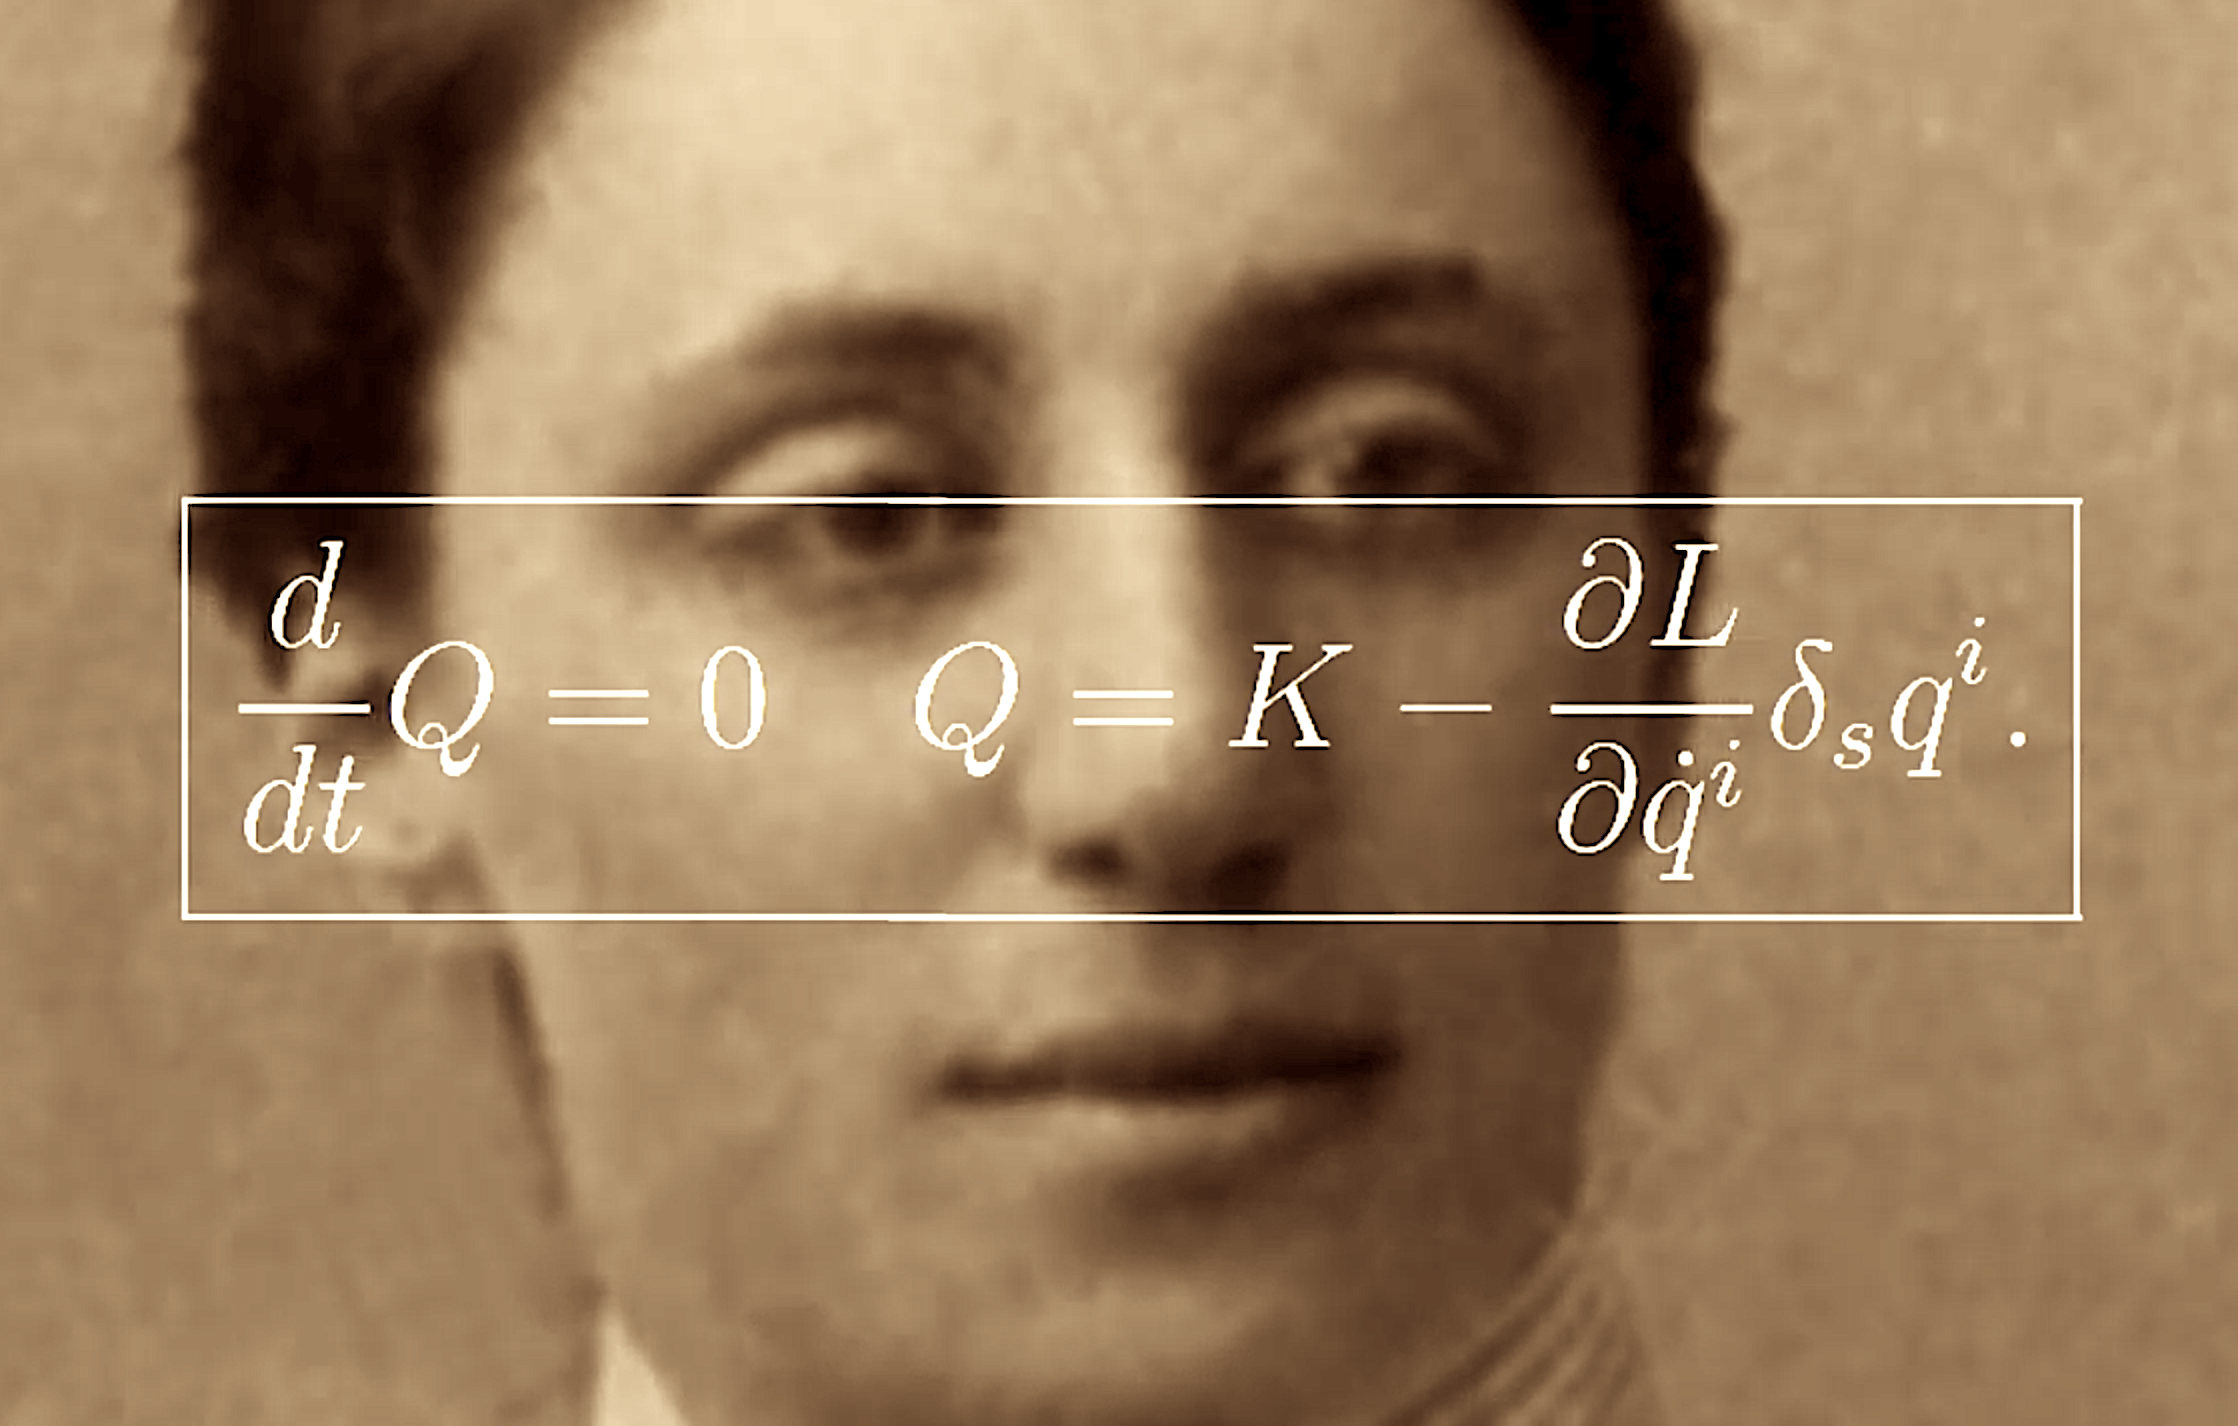
\includegraphics[width=.75\textwidth]{imagenes/img15-05.png}
\end{figure}